\section{Configuration, Data-acquisition, and Calibration Software for the NSW Front-end Electronics}
\label{sec:nsw_vrs}

To facilitate the testing and readout of the VMM ASIC, in view
of its evolution and preparedness for its use in the NSW,
a complete system has been built.

\begin{figure}[!htb]
    \begin{center}
        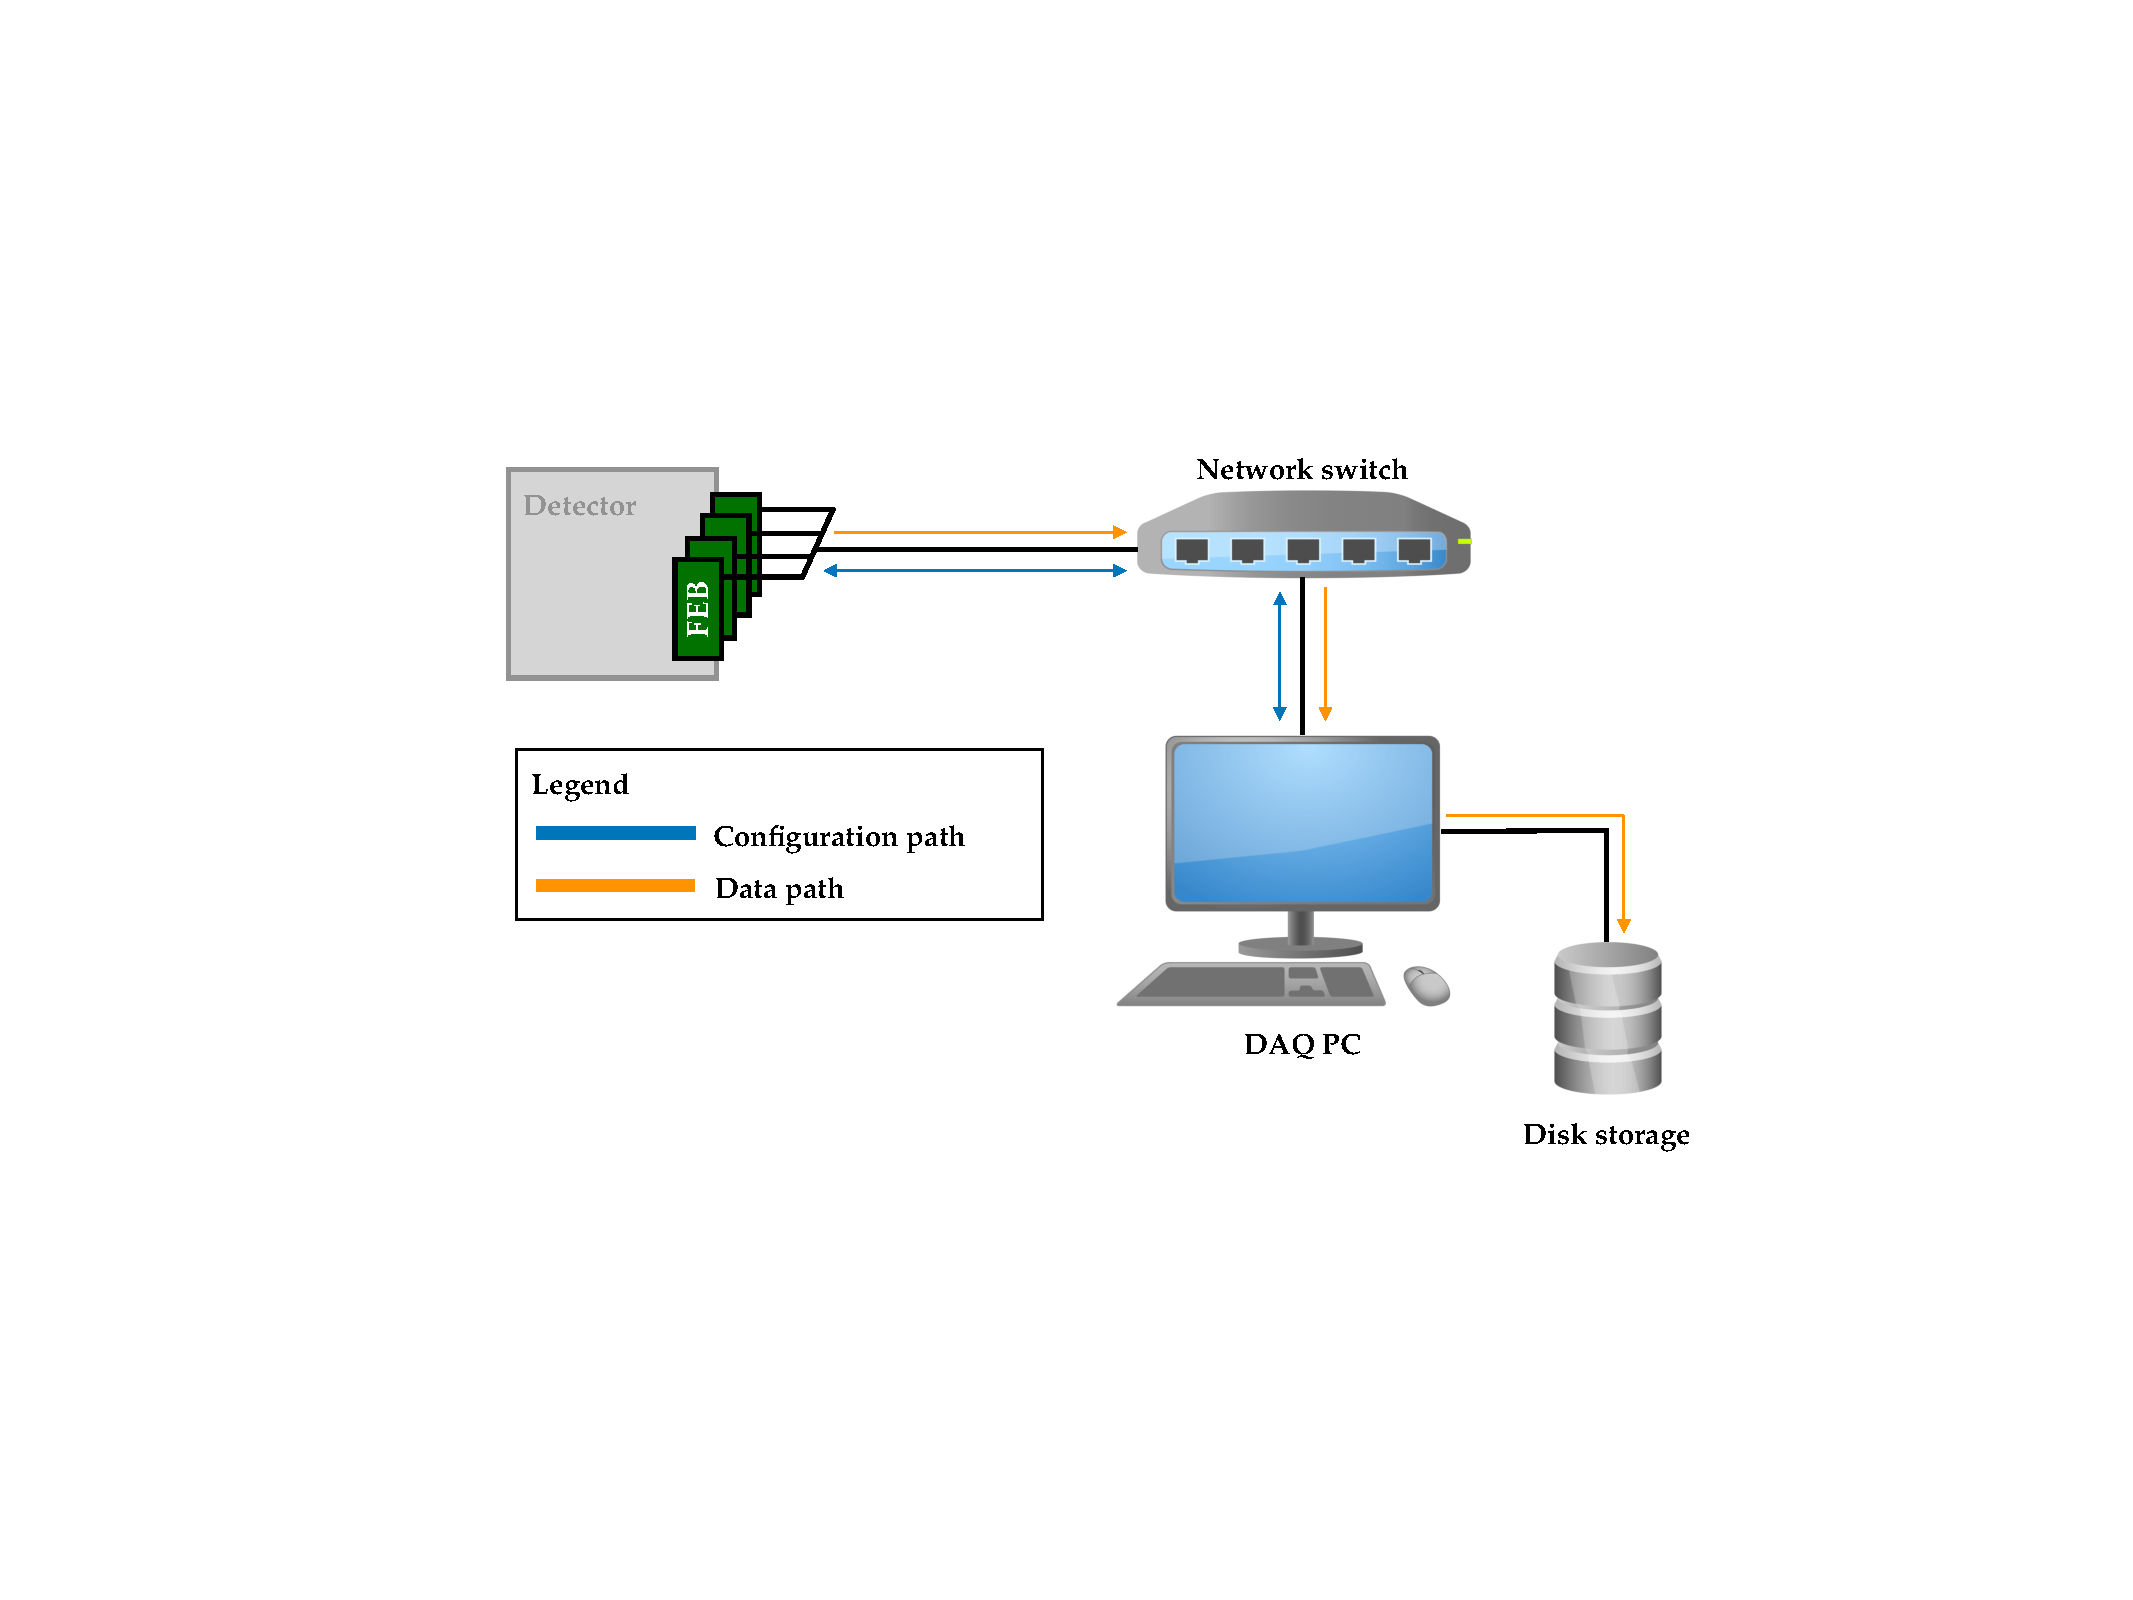
\includegraphics[width=0.5\textwidth]{figures/nsw/vrs/vrs_diagram_minimalPDF}
        \caption{
        }
        \label{fig:vrs_diagram_minimal}
    \end{center}
\end{figure}

\begin{figure}[!htb]
    \begin{center}
        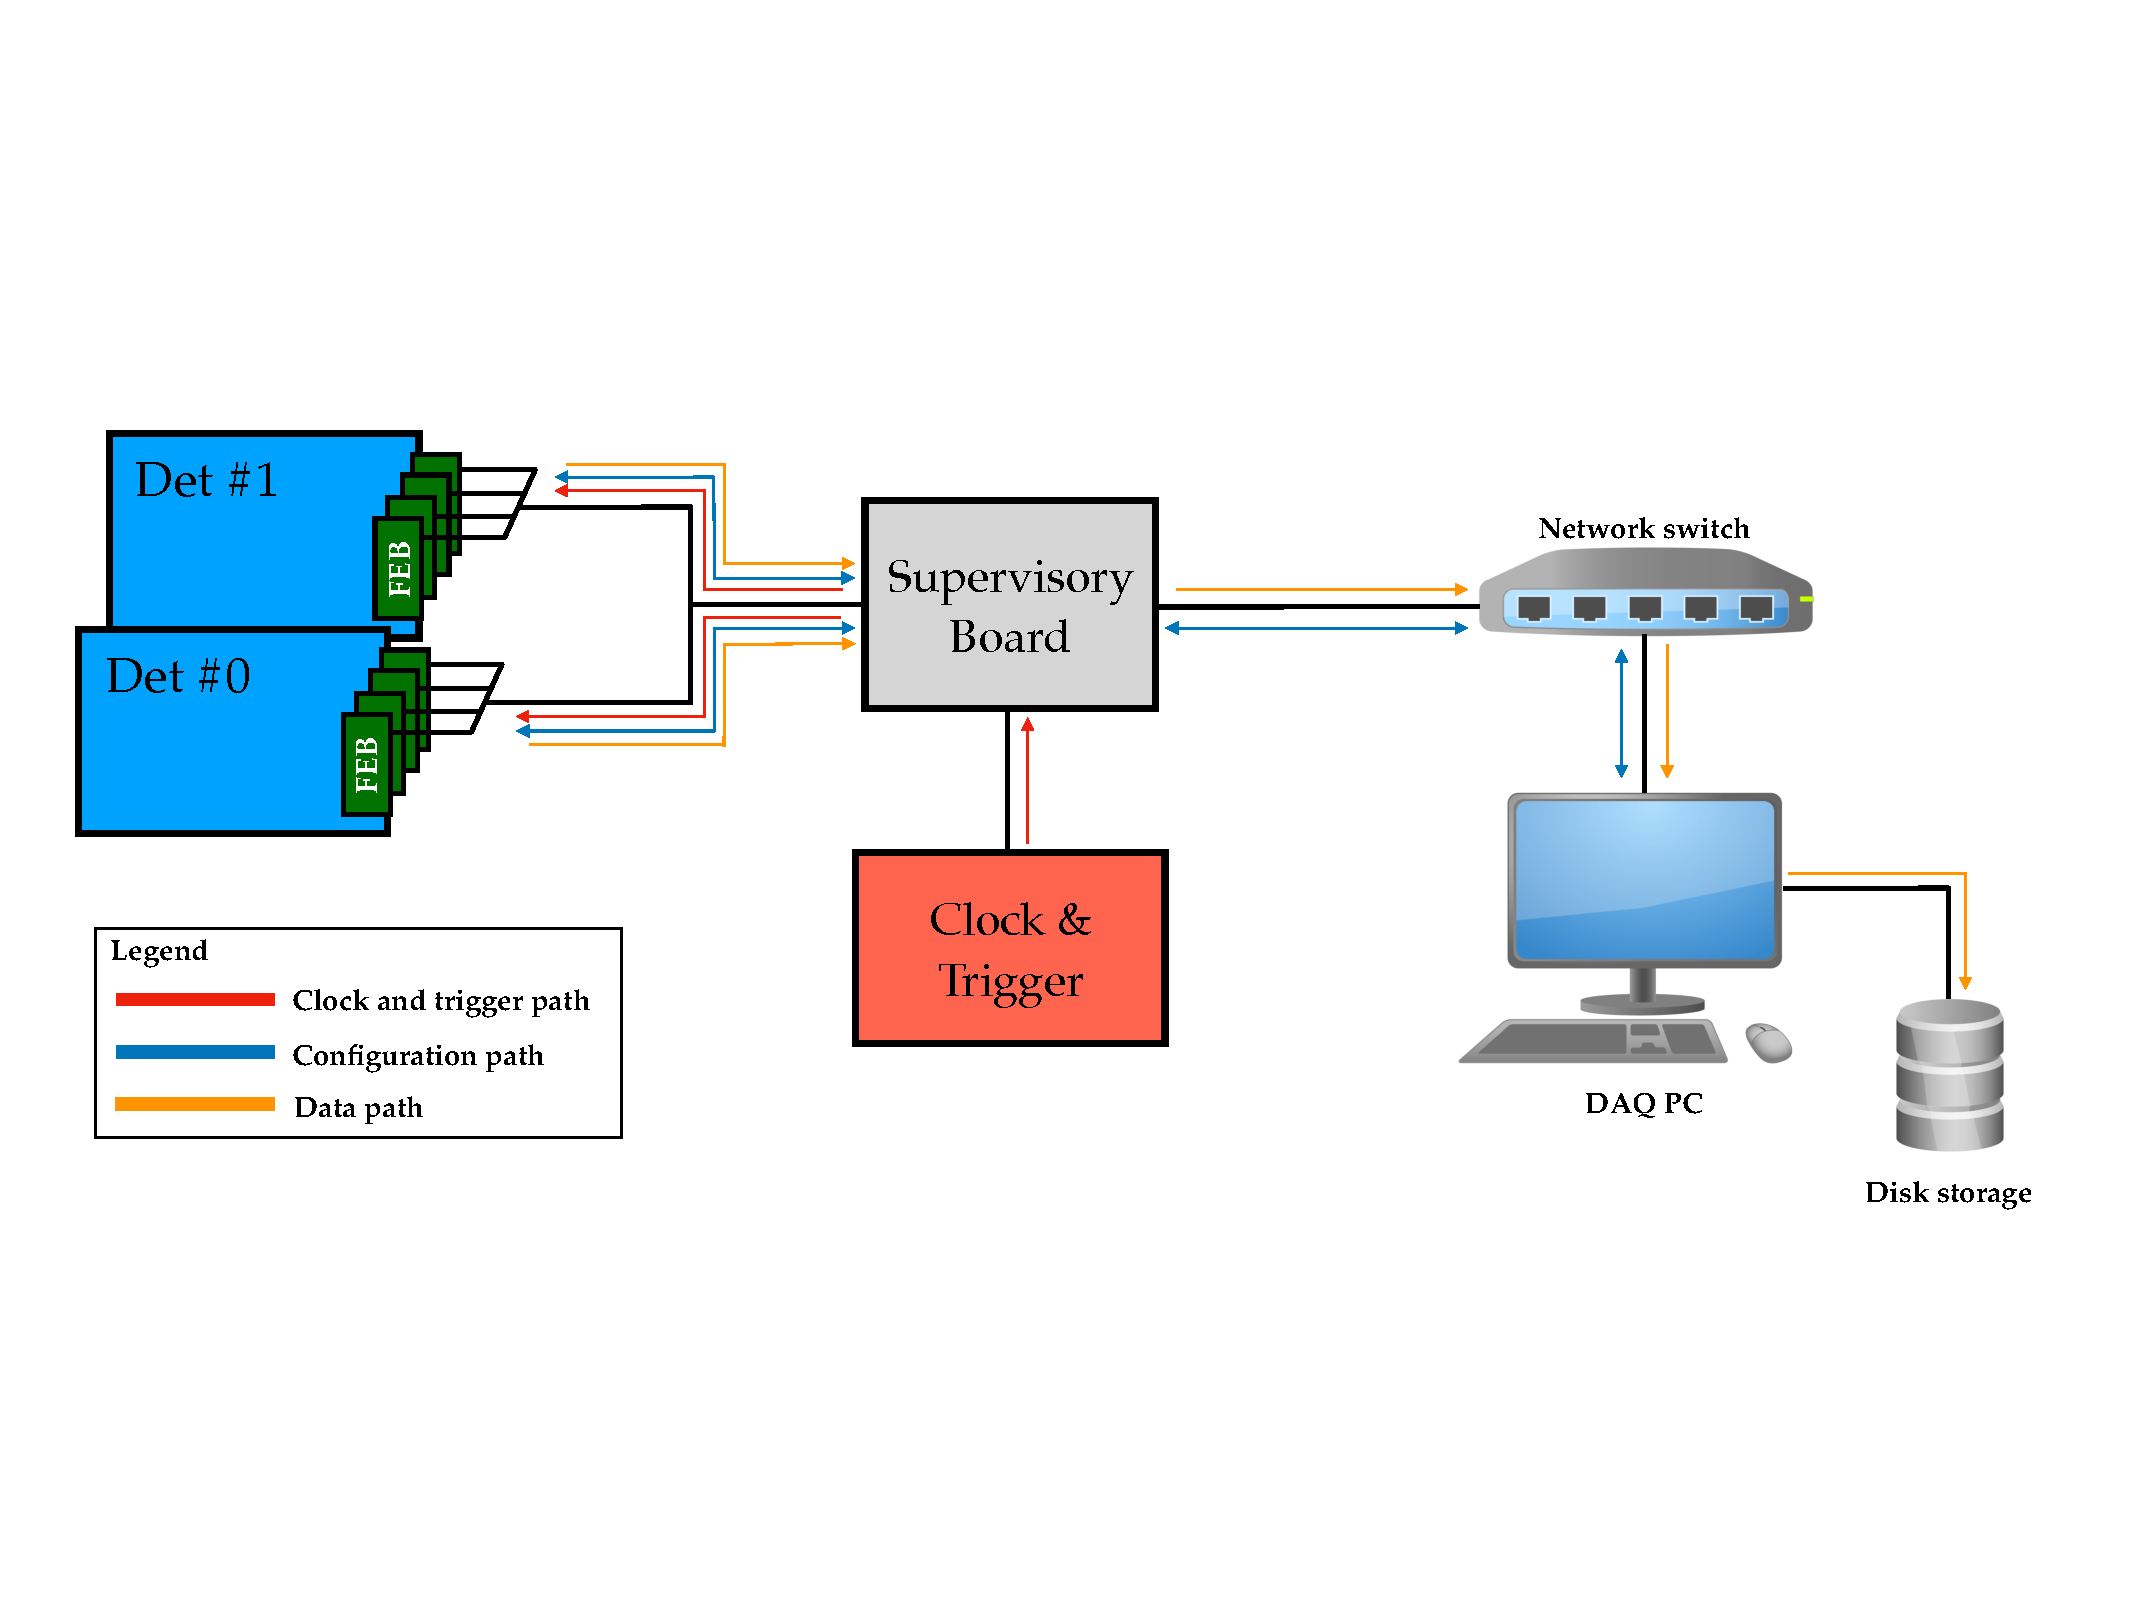
\includegraphics[width=0.7\textwidth]{figures/nsw/vrs/vrs_diagramPDF}
        \caption{
        }
        \label{fig:vrs_diagram}
    \end{center}
\end{figure}

\subsection{VERSO}
\label{sec:verso}

\subsection{Calibration Algorithm Development}
\label{sec:calib_alg}

%\subsubsection{Gain}
%\subsubsection{ADC Calibration}
%\subsubsection{Noise Measurements}
%\subsubsection{Timing Calibration}
%\subsubsection{Per-channel Threshold Equilisation}
